
\section{Design}
\begin{frame}[fragile]
	\frametitle{Class Design: Solution Representation}


	\begin{tikzpicture}
		\node[anchor=north west] at (-1, 4){%
			\parbox{10cm}{%
				\small
				The solution of the corresponding Euler-Lagrange equations
					{%
						\begin{equation*}
							-\alpha_1 \diffk{\qv}{t}{2}+ \alpha_2 \diffk{\qv}{t}{4}- \cdots +  {(-1)}^k \alpha_k \diffk{\qv}{t}{2k}= 0 \ \ \text{a.e.}
						\end{equation*}
					}
			}};

		\only<4>{
			\node[rectangle split, rectangle split allocate boxes=5,
				rectangle split parts=5,
				anchor=north west,
				font=\ttfamily,
				align=left,
				rectangle split part align=left] at (-1, 2) (class) {class GSpline\{
				\nodepart{second}
				\hglue1cm Eigen::VectorXd coefficients\_;
				\nodepart{third}
				\hglue1cm Eigen::VectorXd time\_interval\_lengths\_;
				\nodepart{fourth}
				\hglue1cm Basis basis\_;\\
				\}
			};
			\node[anchor=north,yshift=1cm,xshift=-2cm] at (class.south) {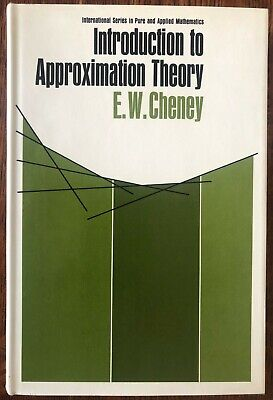
\includegraphics[height=3cm]{./images/cheneybook.jpg}};
			\draw[->] ($(class.two east)-(1.9, 0)$) -- ++(4, 0) node[anchor=west, name=ll]{$[\av_0^1$ \ $\cdots$ \ $\av_{2k}^1\cdots]$};
			\draw[->] (class.three east) -- (class.three east -| ll.west) node[anchor=west]{$[\tau_1\ \cdots \ \tau_{N}]$};
			\draw[->] ($(class.four east)-(5, 0)$) -- (class.four east -| ll.west) node[anchor=west]{$[B_i, \cdots, B_{2k}]$};

		}
		\only<1>{
		\foreach \x/\t in {0/0, 0.6/1, 2/2, 6.9/{N-1},  8.2/{N}} {
		\draw[->] (\x,0.2) -- (\x, 0.5) node[anchor=south]{$\wp_{\t}$};
		}
		\foreach \x/\t in { 3.7/j, 5.1/{j+1}} {
		\draw[->] (\x,-0.7) -- ++(0, -0.3) node[anchor=north]{$\wp_{\t}$};
		}
		\node at (11, 2.7){\parbox{3cm}{\textbf{Unknows}:\\ $t_j$ and $\tau_j$}};
		}
		\only<1-3>{
		% Draw the horizontal line representing the time interval
		\draw[thick,->] (0,0) -- (9,0) ;

		% Label the start of the interval

		% Define the number of sub-intervals
		\foreach \x/\t in {0/{$t_{0}$}, 0.6/{$t_{1}$}, 2/{$t_{2}$}, 3/{$\cdots$}, 3.7/{$t_j$}, 5.1/{$t_{j+1}$}, 6/{$\cdots$}, 6.9/{$t_{N-1}$}, 8.2/{$t_f$} } {
		\node[anchor=north] at (\x,0) {\Large\t};
		}

		\foreach \x/\t in {0, 0.6, 2, 3.7, 5.1, 6.9,  8.2} {
				\draw[thick] (\x,0.1) -- (\x,-0.1);
			}

		\draw[decorate,decoration={brace,amplitude=10pt}] (3.7,0.5) -- (5.1,0.5) node[midway,yshift=0.7cm,name=SolI] {
			\only<2>{$\qv(t)=\sum_{i=1}^{2k} \av^{\ j}_i B_i(t)$}
			\only<1>{$\tau_i = t_{j+1} - t_j$}
		};
		\only<2>{\draw[decorate,decoration={brace,mirror,amplitude=10pt}] (0.6,-0.7) -- (2,-0.7) node[midway,yshift=-0.7cm,name=A] {$\qv(t)=\sum_{i=1}^{2k} \av^{\ 1}_i B_i(t)$}};
		\draw[decorate,decoration={brace,mirror,amplitude=10pt}] (6.9,-0.7) -- (8.2,-0.7) node[midway,yshift=-0.7cm, name=SolN] {
			\only<2>{$\qv(t)=\sum_{i=1}^{2k} \av^{\ 1}_i B_i(t)$}
			\only<1>{$\tau_i = t_{f} - t_{N-1}$}

		};

		\only<2>{%
		\matrix (mymatrix) [matrix of nodes, nodes in empty cells, left delimiter={[}, right delimiter={]}] at (12,1) {
						$\vdots$ \\  $\av_0^j$ \\ $\vdots$ \\ $\av_{2k}^j$ \\ $\vdots$  \\  $\av_0^{N-1}$ \\ $\vdots$ \\ $\av_{2k}^0$ \\
					};
				\draw[decorate,decoration={brace,mirror, amplitude=10pt}] ($(mymatrix-2-1)+(-1, 0.3)$) -- ($(mymatrix-4-1)+(-1, -0.3)$) coordinate[midway, xshift=-0.5, name=I1];
				\draw[thick, ->] (SolI.east) -| ++(2, 0) |- ($(I1.west)+(-0.4,0)$);
				\draw[decorate,decoration={brace,mirror, amplitude=10pt}] ($(mymatrix-6-1)+(-1, 0.3)$) -- ($(mymatrix-8-1)+(-1, -0.3)$) coordinate[midway, xshift=-0.5, name=I1];
				\draw[thick, ->] (SolN.east) -| ++(0.4, 0) |- ($(I1.west)+(-0.4,0)$);
			}
		\only<3>{%
		\matrix (mymatrix) [matrix of nodes, nodes in empty cells, left delimiter={[}, right delimiter={]}] at (12,1) {
						$\tau_0$ \\ $\vdots$ \\  $\tau_j$ \\  $\vdots$ \\ $\tau_{N-1}$  \\
					};
				\draw[thick, ->] (SolI.east) -| ++(2, 0) |- ($(mymatrix-3-1)+(-0.4,0)$);
				\draw[thick, ->] (SolN.east) -| ++(2, 0) |- ($(mymatrix-5-1)+(-0.4,0)$);
			}
		\only<3>{%
			\draw[decorate,decoration={brace,amplitude=10pt}] (0,0.5) -- (0.6,0.5) node[midway,yshift=0.7cm,name=SolI] {};
			\draw[thick, ->] (SolI.south) |- ++(10, 0.8)  |- ($(mymatrix-1-1)+(-0.4,0)$);
		}
		}
	\end{tikzpicture}
	\vfill
\end{frame}


\begin{frame}[fragile]
	\frametitle{Class Design: Overview}

	\begin{columns}
		\begin{column}{0.5\textwidth}
			\begin{lstlisting}[language=c++]
class GSpline {
private:
    Eigen::VectorXd time_interval_lengths_;
    Eigen::VectorXd coefficients_;
    double initial_time_;
    std::unique_ptr<Basis> basis_;
public:
    GSpline linear_scaling_new_execution_time(double _T) const;
    GSpline operator+(const GSpline& that);
    GSpline operator*(double num);
    GSpline derivative(std::size_t deg);
    bool operator()(double time) const;
};
    \end{lstlisting}
		\end{column}
		\begin{column}{0.5\textwidth}
			\begin{lstlisting}[language=C++]
class Basis {
protected:
    Eigen::VectorXd parameters_float_;
    Eigen::VectorXi parameters_int_;
public:
    virtual void eval_on_window(
                    ..., Eigen::VectorXd&_buff) const = 0;
    virtual void eval_derivative_on_window(
                    ..., Eigen::VectorXd& _buff) const = 0;
    virtual void eval_derivative_wrt_tau_on_window(
                    ..., Eigen::VectorXd& _buff) const = 0;

    virtual std::unique_ptr<Basis> clone() const = 0;
};
    \end{lstlisting}
		\end{column}
	\end{columns}
	\begin{center}
		\begin{tikzpicture}[scale=0.9]
			\tikzumlset{font=\fontsize{5}{4}\selectfont}
			\umlemptyclass{GSpline}
			\umlemptyclass[x=7, y=0]{Basis}
			\umlunicompo [angle1=-90, angle2=-140 ] {GSpline}{Basis}
			\umlemptyclass[x=3, y=-2]{BasisLagrange}
			\umlemptyclass[x=6, y=-2]{BasisLegendre}
			\umlemptyclass[x=9, y=-2]{CustomBasis}
			\umlVHVinherit[] {CustomBasis}{Basis}
			\umlVHVinherit[] {BasisLagrange}{Basis}
			\umlVHVinherit[] {BasisLegendre}{Basis}
		\end{tikzpicture}
	\end{center}
\end{frame}

\begin{frame}[fragile]
	\frametitle{Class Design: Bases Implemented}
	\begin{itemize}
		\item Polynomial Basis solution of
		      \begin{eqnarray}
			      \min \int_{t_0}^{t_f} \left\|\diffk{\qv}{t}{k}\right\|^2 \d t
		      \end{eqnarray}
		      \begin{itemize}
			      \item  \Verb|basis::BasisLegendre|
			      \item  \Verb|basis::BasisLagrange|: \\
			            \emphImFusion{Gauss-Radau and Gauss-Lobatto} \tikz[remember picture, overlay]{
				            \node[starburst, draw, minimum width=3cm, minimum height=2cm]
				            at (3.5, 0.5) {\bf Optimal Control!};
			            }
		      \end{itemize}
		\item Non Polynomial basis
		      \begin{eqnarray}
			      \min \int_{t_0}^{t_f} \alpha \left\|\diffk{\qv}{t}{}\right\|^2  + (\alpha - 1 )\left\|\diffk{\qv}{t}{3}\right\|^2 \d t
		      \end{eqnarray}
		      \begin{itemize}
			      \item  \Verb|basis::Basis0101|
		      \end{itemize}
	\end{itemize}
\end{frame}

\begin{frame}[fragile]
	\frametitle{Design: General operations}
	We also desire to work with \emphImFusion{\bf trajectories that are not gsplines}
	\begin{itemize}
		\item The norm of a derivative ${\left\| \ddot \qv \right\|}^2$
		\item Non linear parametrization $ \qv \circ s $, where $\qv, s\in \text{\Verb|GSpline|}$
	\end{itemize}
	For this reason we also provide interface to construct \emphImFusion{general differentiable expressions}
	\begin{itemize}
		\item Scalar \Verb|GSplines| times a vector \Verb|GSpline|
		\item Composition of \Verb|GSplines|
	\end{itemize}
	\begin{center}
		\begin{tikzpicture}[scale=0.9]
			\tikzumlset{font=\fontsize{5}{4}\selectfont}
			\umlemptyclass[x=0, y=0]{FunctionBase}
			\umlemptyclass[x=-3, y=-2]{CustomFunction}
			\umlemptyclass[x=3, y=-2]{FunctionExpression}
			\umlVHVinherit[] {FunctionExpression}{FunctionBase}
			\umlVHVinherit[] {CustomFunction}{FunctionBase}
			\umlHVHunicompo[anchor1=east,angle1=0, arm1=1cm, angle2=0,mult1=1, mult2=1..*] {FunctionExpression}{FunctionBase}
		\end{tikzpicture}
	\end{center}
\end{frame}
\begin{frame}[fragile]
	\frametitle{Design: General Overview}
	\begin{center}
		\begin{tikzpicture}
			\tikzumlset{font=\fontsize{5}{4}\selectfont}
			\umlemptyclass[x=0, y=0]{FunctionBase}
			\umlemptyclass[x=3, y=-2]{FunctionExpression}
			\umlVHVinherit[] {FunctionExpression}{FunctionBase}
			\umlHVHunicompo[anchor1=east,angle1=0, arm1=1cm, angle2=0,mult1=1, mult2=1..*] {FunctionExpression}{FunctionBase}
			\tikzumlset{font=\fontsize{5}{4}\selectfont}
			\umlemptyclass[y=-4]{GSpline}
			\umlemptyclass[x=7, y=-4]{Basis}
			\umlunicompo [angle1=-90, angle2=-140 ] {GSpline}{Basis}
			\umlemptyclass[x=3, y=-6]{BasisLagrange}
			\umlemptyclass[x=6, y=-6]{BasisLegendre}
			\umlemptyclass[x=9, y=-6]{CustomBasis}
			\umlVHVinherit[] {CustomBasis}{Basis}
			\umlVHVinherit[] {BasisLagrange}{Basis}
			\umlVHVinherit[] {BasisLegendre}{Basis}
			\umlVHVinherit[] {GSpline}{FunctionBase}
		\end{tikzpicture}
	\end{center}
\end{frame}

\begin{frame}[fragile]
	\frametitle{Out of the Box Optimization}
	\begin{columns}
		\begin{column}{0.3\textwidth}
			\begin{itemize}
				\item[{\tikz[baseline]{\fill[imfusionBlue] (0,1cm) circle (0.07cm);}}] 
\includegraphics[height=1.6cm]{images/Ipopt.png}
				\vglue1cm
				\item[{\tikz[baseline]{\fill[imfusionBlue] (0,0.5cm) circle (0.07cm);}}] 
\includegraphics[height=0.8cm]{images/ifopt.png}
				{\tiny https://github.com/ethz-adrl/ifopt}
			\end{itemize}
		\end{column}
		\begin{column}{0.7\textwidth}

			\begin{itemize}
				\item We provide custom cost functions and constraints to build
				\item Minimum-X Trajectories
				\item Minimum Time smooth and path consistent collision avoidance
				      % \item For simple gradient based, is it possible to
				      %       \begin{lstlisting}[language=python,
				      % basicstyle=\fontsize{10pt}{0pt}\selectfont\fontfamily{zi4}\selectfont,
				      % ]
				      % import gsplines
				      % alpha=0.1
				      % q=gspliens.GSpline.Zero()
				      % constFunction = MyConstFunction()
				      % while not kktCondtitions(constFunction, q):
				      % q+= alpha*constFunction.diff(q)
				      % \end{lstlisting}

			\end{itemize}
		\end{column}
	\end{columns}
\end{frame}


\begin{frame}[fragile]
	\frametitle{Optimization: Trajectory Generation}
	\begin{columns}
		\begin{column}{0.4\textwidth}
			\begin{lstlisting}[language=python]

waypoints = np.random.rand(4, 2)

straigh_lines = broken_lines_path(waypoints)
min_acc = minimum_acceleration_path(waypoints)
min_jerk = minimum_jerk_path(waypoints)
min_snap = minimum_snap_path(waypoints)
min_crackle = minimum_crackle_path(waypoints)

plot2d_compare([straigh_lines, min_acc, min_jerk, min_snap, min_crackle], [
            'green', 'blue', 'magenta', 'red', 'black'],
            ['min vel', 'min acceleration', 'min jerk',
            'min snap', 'min crackle'])

time_1 = 0.1
time_2 = 0.3

values_at_times = cq(np.array([time_1, time_2]))

vel_norm = min_jerk.deriv(1).dot(min_jerk.deriv(1))
plot(vel_norm)
    \end{lstlisting}
		\end{column}
		\begin{column}{0.6\textwidth}
			\begin{tikzpicture}[scale=1, transform shape]
				\node (pic) {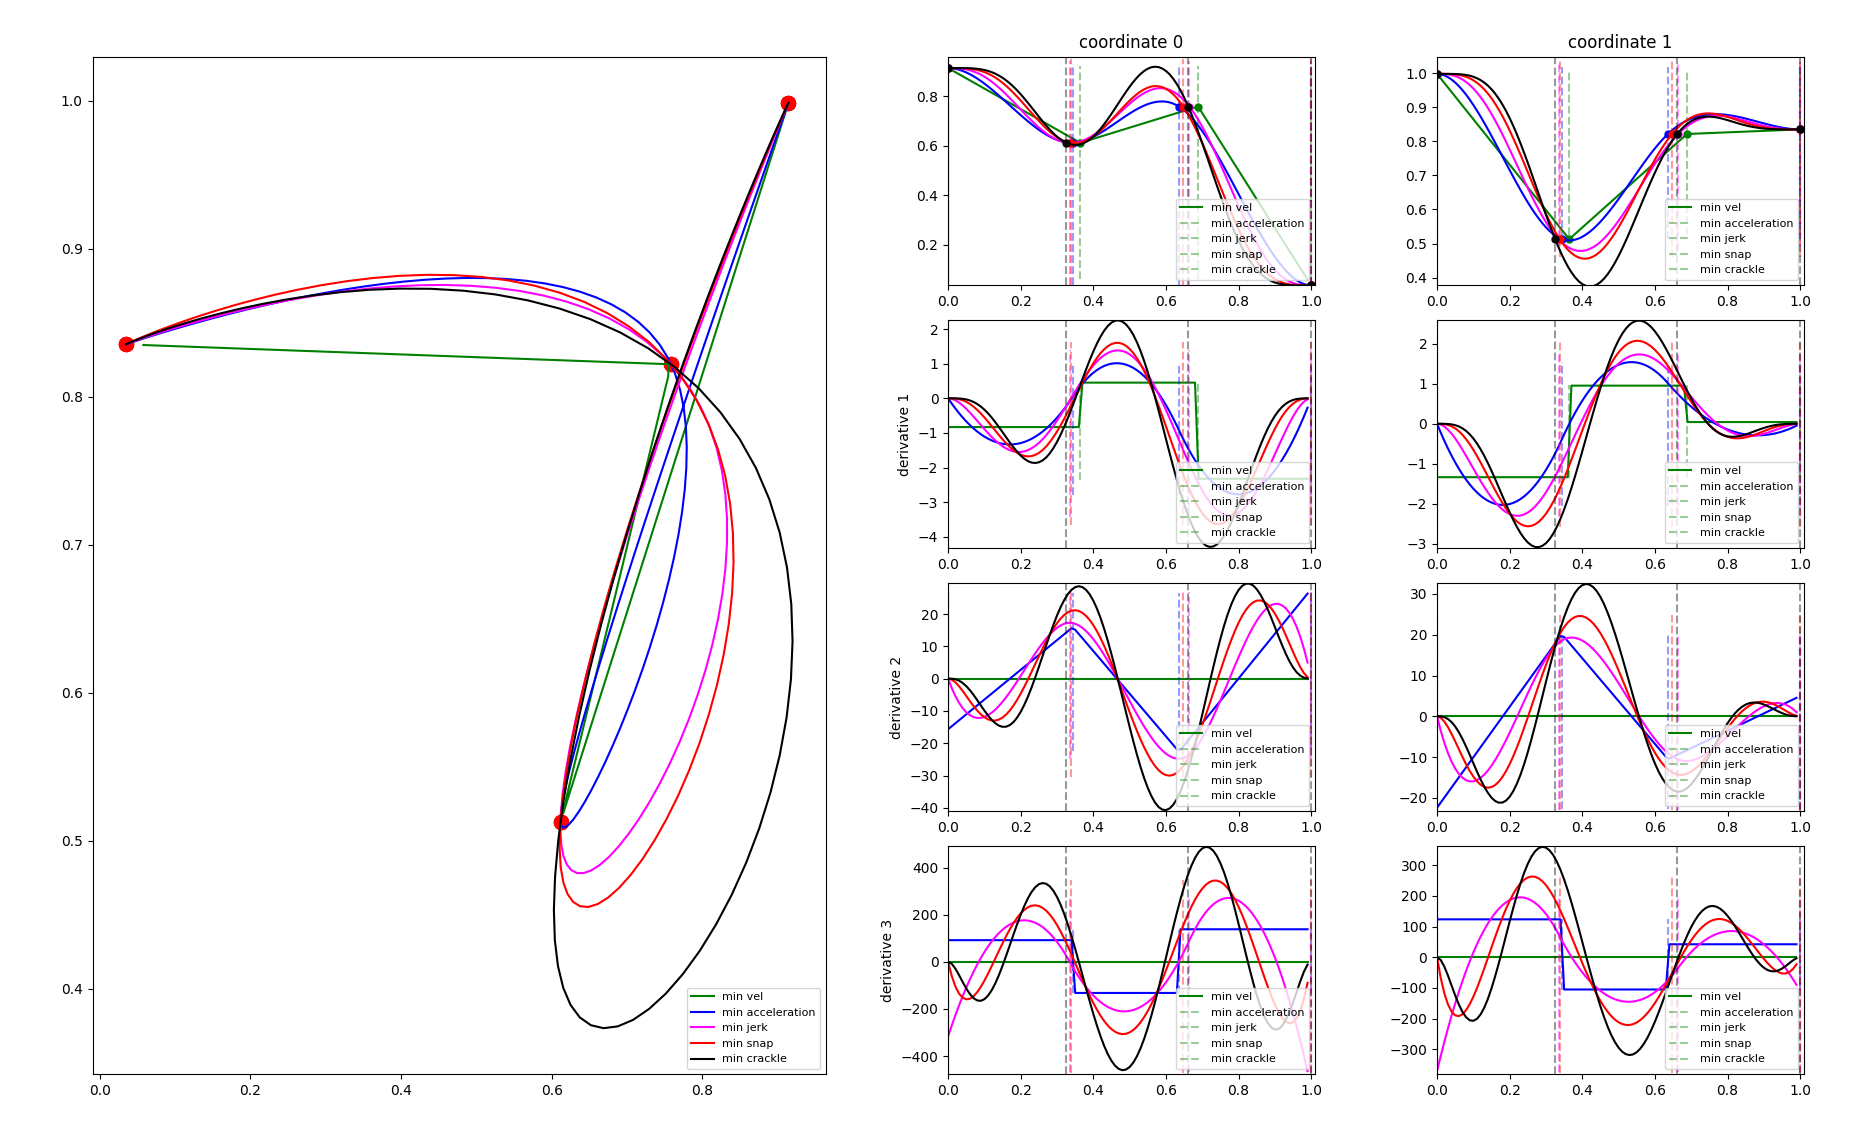
\includegraphics[width=\textwidth]{./images/comparison.png}};
				\node[anchor=north] (qd) at (pic.south) {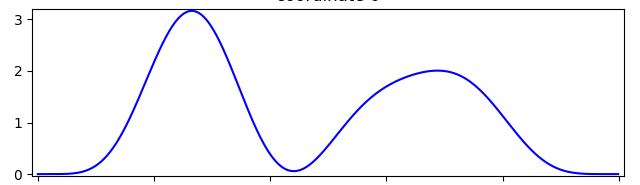
\includegraphics[width=0.7\textwidth]{./images/qd_norm.png}};
				\node[anchor=east] at (qd.west) {$\|\dot{q}\|$};
			\end{tikzpicture}
		\end{column}
	\end{columns}

\end{frame}

\begin{frame}[fragile]
	\frametitle{Optimization: Parametrization Generation.}
	\framesubtitle{Minimum time stop for collision avoidance}
	\begin{columns}
		\begin{column}{0.4\textwidth}
			\begin{lstlisting}[language=python,
            ]
import gsplines
import gsplines.plot as gplot
import numpy as np
import opstop
from gsplines.optimization import minimum_jerk_path


model_file = 'path_to_urdf_robot_description'

dim = 7   # number of joints of the robot
# Generate a random numpy array of wayponts
# (each row is a waypoint in R^n)
number_of_waypoints = 5
waypoints = np.random.rand(number_of_waypoints, dim)
# The a minimum jerk trajectory with execution time of 5s
trj = minimum_jerk_path(waypoints)
# Select the time to stop as the 60% of the time.
stop_ti = trj.get_domain()[1]*0.6
# Get a parametrization that minimizes the time and  does not
# allow an increment in the acceleration larger than 50%
optimal_parametrization = \
    opstop.minimum_time_bounded_acceleration(
    trj, stop_ti, 1.5, str(model_file), 8)
# Obtain the stopping trajectory
stop_trj = trj.compose(optimal_parametrization)
# Plot the nominal and the stopping trajectory
gplot.plot_compare([stop_trj, trj], ['red', 'blue'], [
                'Emergency Stop Trajectory',
                'Original Trajectory'], 
                _show=True, _up_to_deriv=2)
    \end{lstlisting}
		\end{column}
		\begin{column}{0.6\textwidth}
			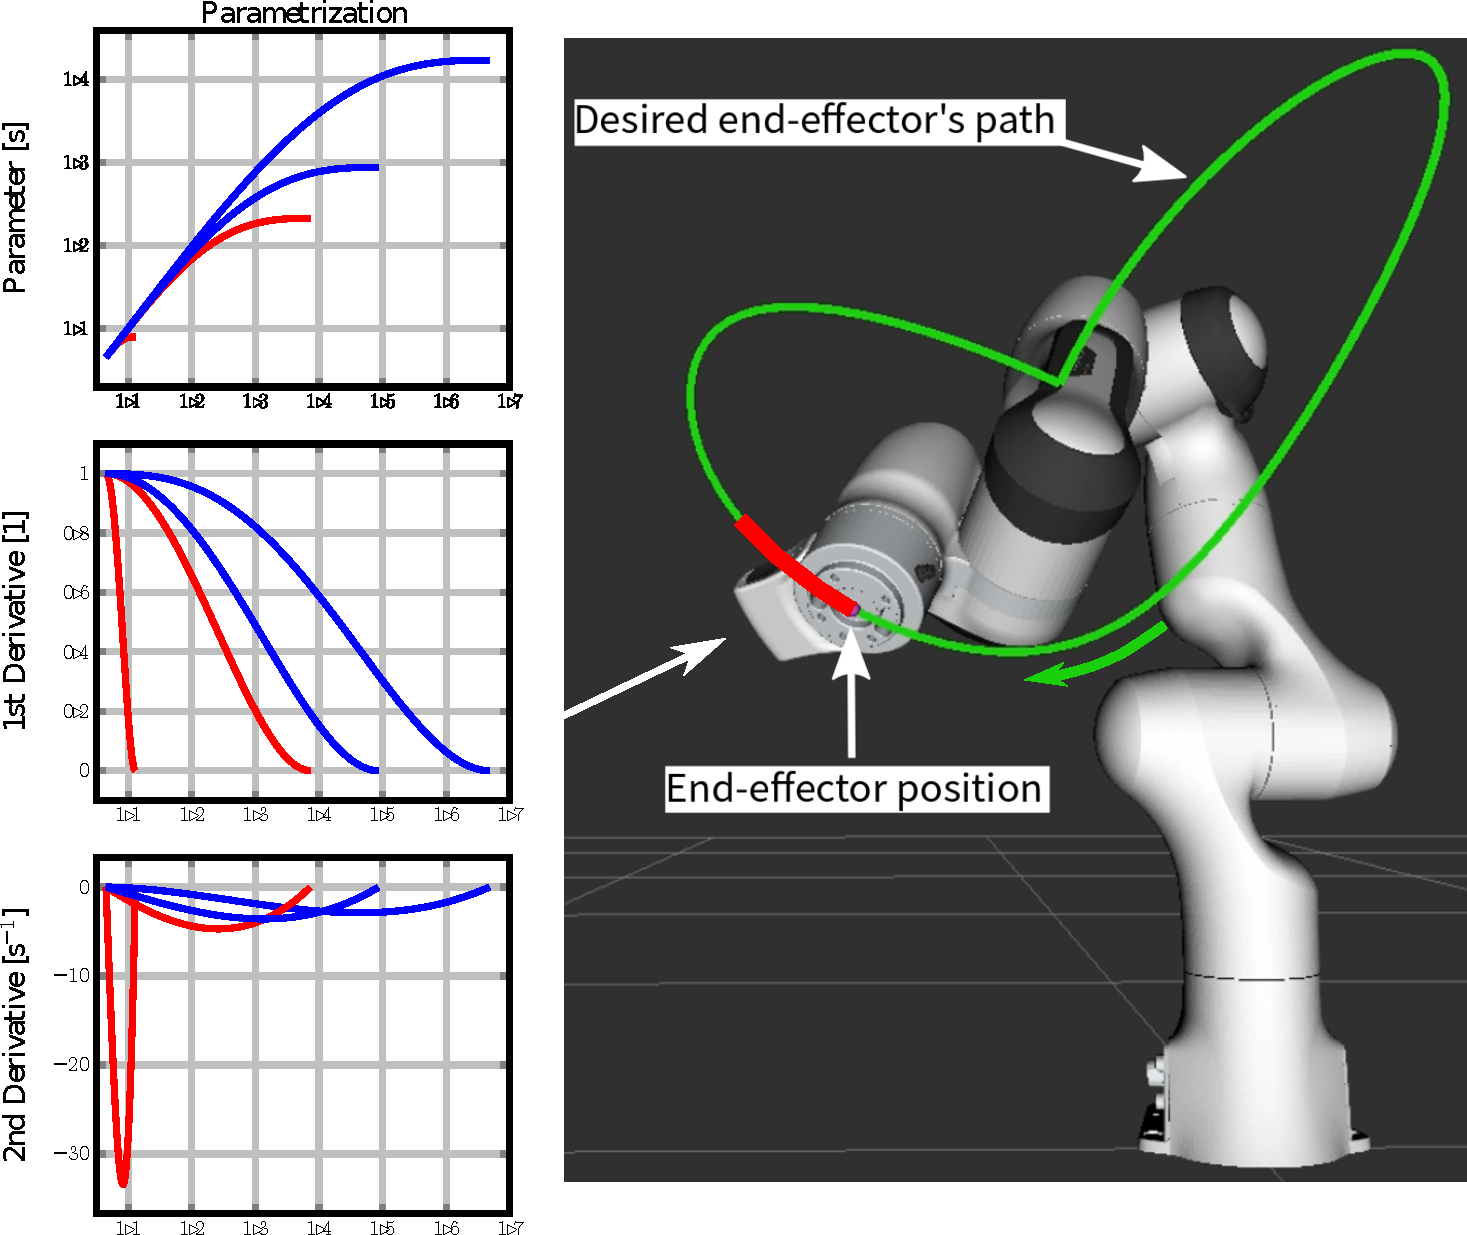
\includegraphics[width=\textwidth]{./images/opstop_param.pdf}
		\end{column}
	\end{columns}
\end{frame}

\begin{frame}[fragile]
	\frametitle{Optimization: Minimum Time Stop.}
	\framesubtitle{Comparison with \Verb|ros\_control| default stop}

	\vglue -1cm
	\begin{columns}
		\begin{column}{0.5\textwidth}
			\begin{tikzpicture}[scale=1, transform shape]
				\node (joints){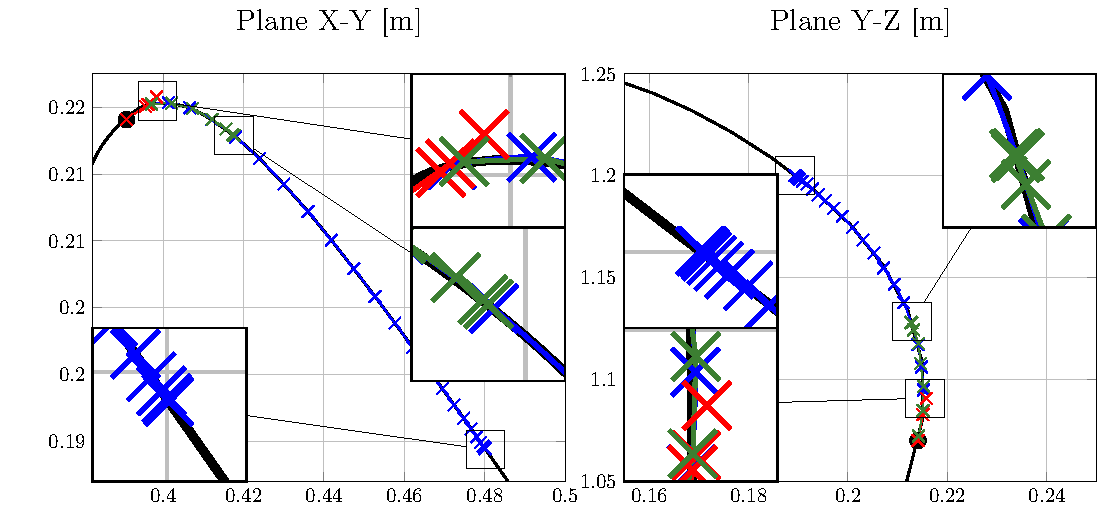
\includegraphics[height=3cm]{./images/opstop_path.pdf}};
				\node[anchor=north east] (j2) at (joints.south east) {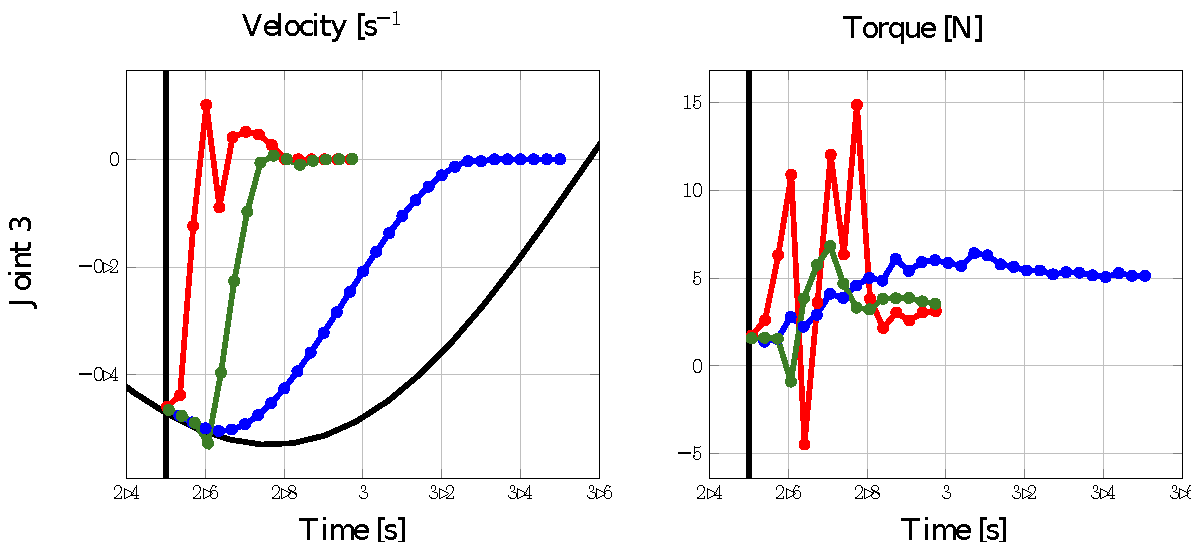
\includegraphics[height=2cm]{./images/opstop_joints.pdf}};
				\node[anchor=east] at (j2.west) {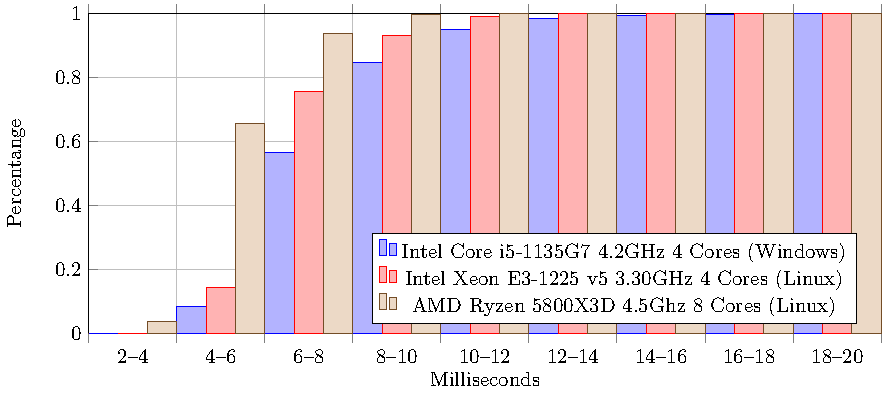
\includegraphics[height=1.4cm]{./images/opstop_time.pdf}};
			\end{tikzpicture}

		\end{column}
		\begin{column}{0.5\textwidth}

		\end{column}
	\end{columns}

\end{frame}


\begin{frame}[fragile]
	\frametitle{Optimization: Minimum Time parametrization.}
	\framesubtitle{Fast and Smooth: Min. Time on a \Verb|GSpline|}
	\begin{tikzpicture}[scale=1, transform shape]
		\node (pic) {
\includegraphics[width=6cm]{./images/mintimepaper.png}};
		\node[anchor=north east]  at (pic.south) {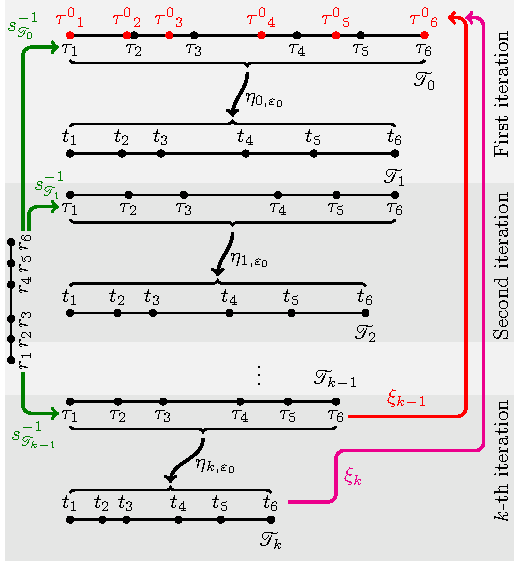
\includegraphics[width=3cm]{./images/mintimeiteration.pdf}};
		\node[anchor=north west] (vel) at (pic.south) {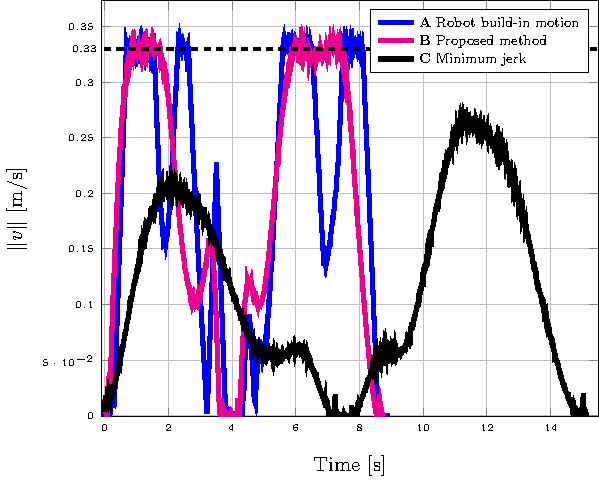
\includegraphics[width=3cm]{./images/mintimevelocity.pdf}};
		\node[anchor=west,xshift=10mm]  at (vel.east) {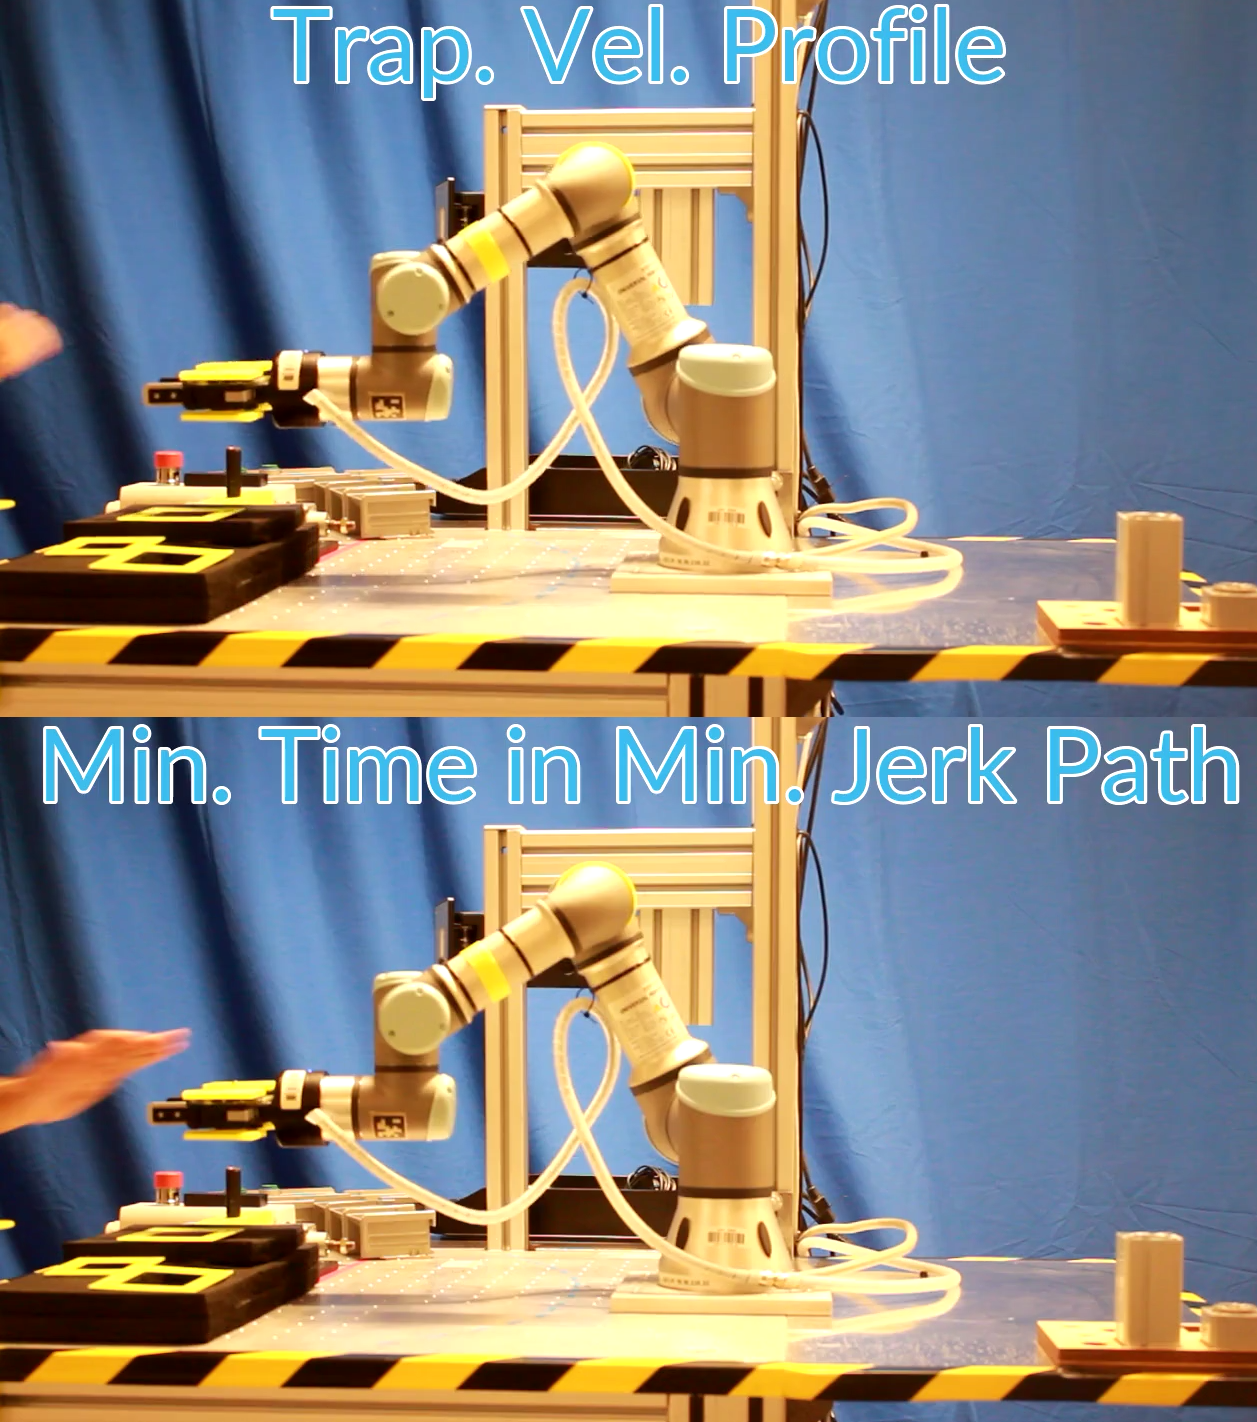
\includegraphics[width=6cm]{./images/mintimevideopreview.png}};

	\end{tikzpicture}

\end{frame}

\begin{frame}[fragile]
	\frametitle{Optimization: Minimum Time Trajectory Planning.}
	\begin{columns}
		\begin{column}{0.5\textwidth}

		\end{column}
		\begin{column}{0.5\textwidth}

		\end{column}
	\end{columns}
\end{frame}
